\subsection{Partes} \label{subsec:partes}
En esta sección se presentan los componentes principales del robot, enfocándose en los motores y los eslabones que forman su estructura. Se describe brevemente el papel que desempeña cada uno dentro del sistema, destacando su importancia en el movimiento, la transmisión de fuerzas y el cumplimiento de las tareas asignadas al robot.


\subsubsection{Motores} \label{subsubsec:motores}

En este proyecto se utilizaron tres tipos de motores, cada uno seleccionado de acuerdo con las necesidades específicas de torque, velocidad y precisión. El primero es un motor paso a paso NEMA 17, que de acuerdo con su hoja de datos entrega un torque máximo de 59 N·cm, equivalente a 0.59 N·m. La velocidad máxima considerada para este motor es de 1000 rpm, que corresponde a 2.65 rad/s. Este motor está conectado a una transmisión con una relación de reducción de 8:1, lo que significa que por cada ocho vueltas del motor, la salida da una vuelta. Los motores NEMA 17 son comúnmente usados en impresoras 3D y pequeñas máquinas CNC, debido a su precisión y control fino de pasos.

El segundo motor utilizado es un paso a paso NEMA 23, que tiene un torque máximo de 1.26 N·m y alcanza una velocidad de hasta 1500 rpm, equivalente a 3.98 rad/s. Este motor está acoplado a un reductor con relación 10:1, permitiendo aumentar el torque a costa de reducir la velocidad, lo que lo hace adecuado para aplicaciones que requieren mayor fuerza, como sistemas actuadores más grandes.



\subsubsection{Eslabones} \label{subsubsec:eslabones}


Para calcular las propiedades físicas de los eslabones del robot, se utilizaron los datos obtenidos de la configuración de las uniones (joints), en particular las posiciones de origen de cada una. Estas posiciones permiten determinar la longitud aproximada de cada eslabón al observar el desplazamiento relativo entre las articulaciones consecutivas. A partir de estas longitudes, y asumiendo que los eslabones tienen forma cilíndrica con un diámetro aproximado de 2.5 cm, fue posible estimar su volumen. Para este proyecto se empleó como material el ABS, un plástico común en impresión 3D y prototipado rápido, que ofrece buena resistencia mecánica y bajo peso, con una densidad aproximada de 1040 kg/m³.

En lugar de estimar la masa, se utilizaron directamente los valores de masa obtenidos para cada eslabón, ya que fueron extraídos de los modelos físicos. Con esta masa y la longitud correspondiente, también se estimó el momento de inercia usando la fórmula I = (1/12)·m·L², correspondiente a un cilindro delgado girando alrededor de su centro.

De esta manera, se obtuvieron los siguientes resultados para cada eslabón:

El \textbf{eslabón 1}, con una masa de 6.19 kg, representa uno de los segmentos estructurales principales del robot. \autoref{fig:joint1urdf}.
El \textbf{eslabón 2} tiene una masa de 8.13 kg y soporta una parte importante de la carga y el movimiento.\autoref{fig:joint2urdf}.
El \textbf{eslabón 3} presenta una masa de 6.53 kg y forma parte del brazo intermedio del robot. \autoref{fig:joint3urdf}.
El \textbf{eslabón 4} tiene una masa de 1.85 kg y corresponde a una sección final más ligera del brazo. \autoref{fig:joint4urdf}.
Finalmente, el \textbf{eslabón 5}, con una masa de 0.59 kg, es el más liviano y está asociado generalmente al extremo del manipulador, como una pinza o herramienta.

Además, la base del robot cuenta con una masa de 10.87 kg, lo cual proporciona la estabilidad necesaria para sostener toda la estructura y resistir los movimientos del brazo robótico durante su operación.

Estos valores permiten aproximar de forma precisa el comportamiento físico del robot en simulaciones dinámicas, facilitando su análisis en contextos de control, planificación y operación.


\begin{figure}
	\centering
	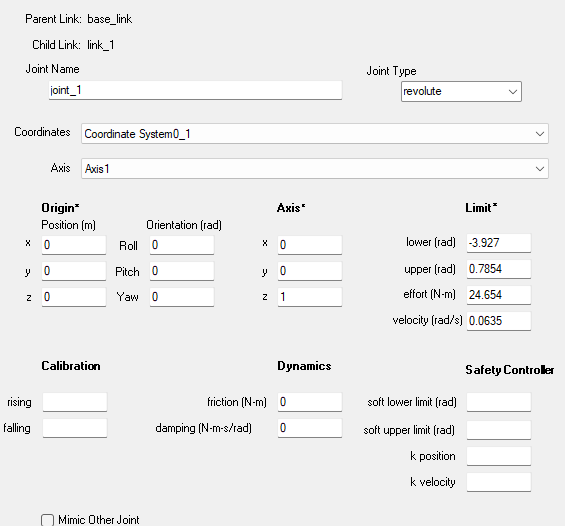
\includegraphics[width=0.3\linewidth]{img/JOINT1URDF}
	\caption{Eslabón 1}
	\label{fig:joint1urdf}
\end{figure}

\begin{figure}
	\centering
	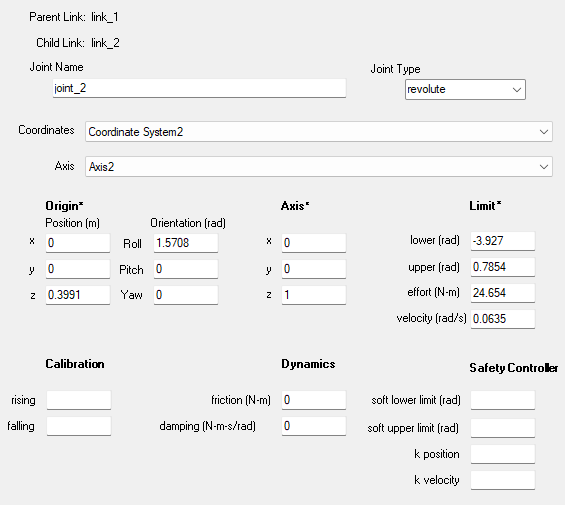
\includegraphics[width=0.3\linewidth]{img/JOINT2URDF}
	\caption{Eslabón 2}
	\label{fig:joint2urdf}
\end{figure}

\begin{figure}
	\centering
	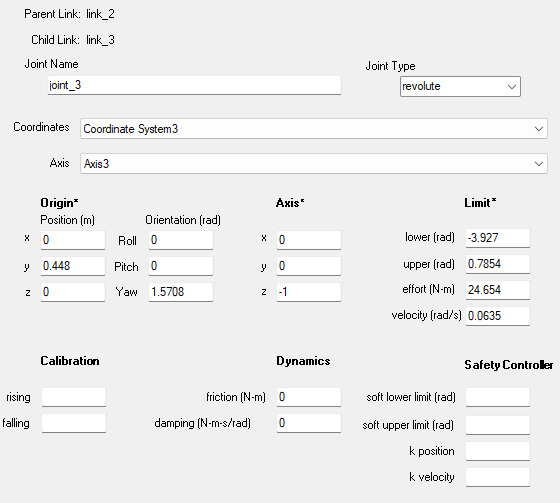
\includegraphics[width=0.3\linewidth]{img/JOINT3URDF}
	\caption{Eslabón 3}
	\label{fig:joint3urdf}
\end{figure}}

\begin{figure}
	\centering
	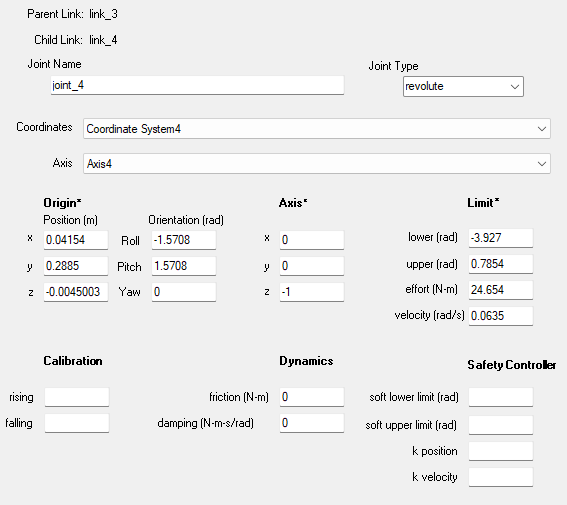
\includegraphics[width=0.3\linewidth]{img/JOINT4URDF}
	\caption{Eslabón 4}
	\label{fig:joint4urdf}
\end{figure}



	





